% ============================================================
% DIAGRAM: Hopfield Network (1982)
% ============================================================
% Caption: Figure 3.3: Hopfield network with symmetric weights.
%          (Adapted from Hopfield, 1982, p. 2555)
% ============================================================

\documentclass[tikz,border=10pt]{standalone}
\usepackage{tikz}
\usepackage{amsmath}
\usepackage{amsfonts}

\usetikzlibrary{shapes,arrows,positioning,fit,calc,backgrounds}

\begin{document}

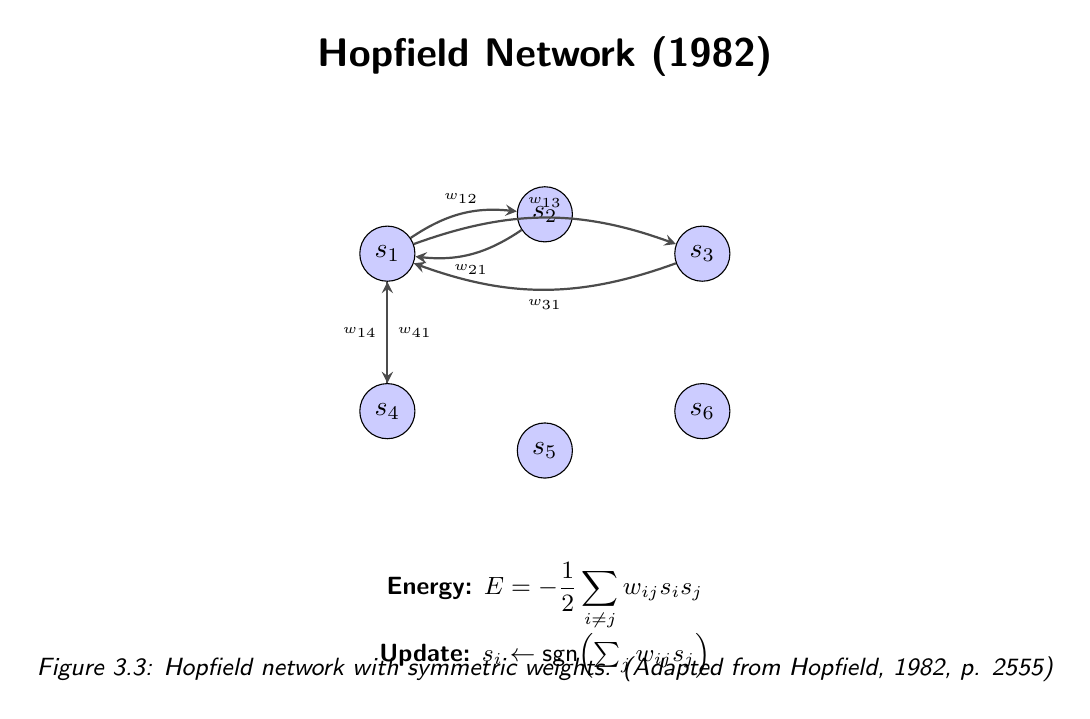
\begin{tikzpicture}[
    neuron/.style={draw, circle, minimum size=0.7cm, inner sep=0pt, fill=blue!20},
    edge/.style={-stealth, thick, draw=black!70},
    label/.style={font=\sffamily\small},
    title/.style={font=\sffamily\Large\bfseries},
    caption/.style={font=\sffamily\small\itshape},
]

\node[title] at (0, 3.5) {Hopfield Network (1982)};

% Neurons
\node[neuron] (n1) at (-2, 1) {$s_1$};
\node[neuron] (n2) at (0, 1.5) {$s_2$};
\node[neuron] (n3) at (2, 1) {$s_3$};
\node[neuron] (n4) at (-2, -1) {$s_4$};
\node[neuron] (n5) at (0, -1.5) {$s_5$};
\node[neuron] (n6) at (2, -1) {$s_6$};

% Fully connected (symmetric) with bidirectional arrows
\draw[edge, bend left=20] (n1) to node[above, font=\tiny] {$w_{12}$} (n2);
\draw[edge, bend left=20] (n2) to node[below, font=\tiny] {$w_{21}$} (n1);

\draw[edge, bend left=20] (n1) to node[above, font=\tiny] {$w_{13}$} (n3);
\draw[edge, bend left=20] (n3) to node[below, font=\tiny] {$w_{31}$} (n1);

\draw[edge] (n1) -- node[left, font=\tiny] {$w_{14}$} (n4);
\draw[edge] (n4) -- node[right, font=\tiny] {$w_{41}$} (n1);

% etc. (simplified: just show a few connections for clarity)

% Energy function
\node[align=center, font=\sffamily\small, anchor=north] at (0, -2.8) {
  \textbf{Energy:} $\displaystyle E = -\frac{1}{2} \sum_{i \neq j} w_{ij} s_i s_j$ \\
  \textbf{Update:} $s_i \leftarrow \text{sgn}\!\left( \sum_j w_{ij} s_j \right)$
};

\node[caption, anchor=north] at (0, -4.0) {
  Figure 3.3: Hopfield network with symmetric weights. (Adapted from Hopfield, 1982, p. 2555)
};

\end{tikzpicture}
\end{document}
